
%(BEGIN_QUESTION)
% Copyright 2006, Tony R. Kuphaldt, released under the Creative Commons Attribution License (v 1.0)
% This means you may do almost anything with this work of mine, so long as you give me proper credit

An operator calls you (the instrument technician) over to look at a liquid receiver tank.  She says the tank is empty, as indicated by the sightglass level gauge (LG) on the side of the tank.  This is a problem, because the level control system is supposed to maintain liquid level at the half-way (50\% full) point:

$$\includegraphics[width=15.5cm]{i01492x01.eps}$$

The first thing you do is look at the position of the control valve, because it is located very close to the level gauge where you and the operator are standing.  You can see that the control valve is wide open.

\vskip 10pt

This is not a new control system.  In fact, it was operating just fine a few days ago.  Identify two different instrument faults that could cause this problem to occur, and explain {\it why} each of those faults would cause this to happen.  

\vfil

\underbar{file i01492}
\eject
%(END_QUESTION)





%(BEGIN_ANSWER)

This is a graded question -- no answers or hints given!

%(END_ANSWER)





%(BEGIN_NOTES)

If we are to trust the sightglass (these have been known to fail!) telling us that the vessel's level is running much too low, we may conclude that the control valve should {\it not} be wide-open like it is.  Either the control valve is being told (incorrectly) to open wide, or its failed open for some reason.

\vskip 10pt

{\bf Some possible faults include:}

\begin{itemize}
\item{} Controller left in manual, 100\% output.  {\it This would cause the valve to open up all the way, and not respond automatically to the resulting decrease in liquid level.}
\vskip 10pt
\item{} Transmitter failed high (telling the controller the tank is completely full).  {\it This would make the controller think it needed to drain liquid from the vessel, causing it to react by opening the valve fully.}
\vskip 10pt
\item{} Controller output faulted with 20+ mA  output.  {\it This would drive the valve to its wide-open position.}
\vskip 10pt
\item{} Valve positioner faulted, forcing valve all the way open.  {\it This would drive the valve fully open even if the controller output was not telling it to open wide.}
\vskip 10pt
\item{} Nozzle plugged in I/P transducer, sending full pressure to valve positioner.  {\it A plugged nozzle in the I/P will cause the backpressure to rise uncontrollably, forcing the I/P's output to saturate high even if its electrical signal in is not high.}
\vskip 10pt
\item{} Someone switched the controller from direct action to reverse.  {\it Assuming a direct-acting transmitter and a signal-to-open control valve, the controller should be configured for direct action as well.  However, if the controller were set to reverse action, it would cause the PV to saturate in one direction rather than stabilize at setpoint like it should.  Interestingly, this fault could just as likely cause the level to saturate high (overfill).  It should be noted that this fault is unlikely, as anyone guilty of switching the controller's action would probably see the immediate effects of their mistake.  Since this was known to be a working system a few days ago, switched controller action becomes an unlikely possibility.}
\end{itemize}

%INDEX% Basics, control loop troubleshooting: determining cause of control problem
%INDEX% Process: receiver vessel liquid level control (generic)

%(END_NOTES)


